% -*- root: 00-main.tex -*-



%{\color{red} {The main diverging points with respect to
%\citep{gorthi_active_2011} are: 1) there is no need for an explicit level set function
%$\Phi_G$, as we replace the level set gradient computation $N_{\Phi_G}$ with shape
%gradients \citep{besson_dream2s_2003,herbulot_segmentation_2006};
%2) regularization is also based on linear diffusion smoothing \citep{thirion_image_1998},
%but we replace the Gaussian filtering by other constraints
%studied in \citep{nagel_investigation_1986} to better the problem;
%3) optimization is applied in the spectral
%domain, observing anisotropic and inhomogeneous mappings along each direction.
%With respect \citep{guyader_combined_2011}, the main differences are
%the distance function, and the spectral solution to the optimization updates,
%as we shall cover in \autoref{sec:numerical_implementation}.}}



%In this paper we formulate the joint registration-segmentation
%problem as follows.
%such that the known contours in anatomical space $T$ optimally segment
%the diffusion space $D$.
%
%
%Whereas related \glspl*{adf} introduced in \autoref{sec:methods_background}
%make use of explicit level-set formulations to solve \eqref{eq:gradient_descent},
%we alternatively use \emph{shape-gradients}
%\cite{besson_dream2s_2003,herbulot_segmentation_2006}.

%
%Let us denote by $\vec{x}$ the voxel and $F(\vec{x}) = [ f_1, f_2, \ldots, f_N]^T$
%  its associated feature vector in the following.
%
%In our application, these surfaces are precise tissue interfaces of interest extracted
%  from a high-resolution, anatomically correct reference volume using
%  the well-established
%
%In this paper we propose a novel registration framework to simultaneously
%solving the segmentation, distortion and cortical parcellation challenges,
%by exploiting as strong shape-prior the detailed morphology extracted
%from high-resolution and anatomically correct \gls{mri}.
%Indeed, hereafter
%we assume this segmentation problem in anatomical images is reliably and
%accurately solved with readily available tools (e.g.
%\citep{fischl_freesurfer_2012}).
%After global alignment with \gls{t1} using existing approaches, the remaining
%spatial mismatch between anatomical and diffusion space is due to susceptibility
%distortions.
%Finally, we need to establish precise spatial correspondence between the
%surfaces in both spaces, including the tangential direction for parcellation.
%Therefore, we can reduce the problem to finding the differences of spatial
%distortion in between anatomical and \gls{dwi} space.
%We thus reformulate the segmentation problem as an inverse problem, where we
%seek for an underlying deformation field (the distortion) mapping
%from the structural space into the diffusion space, such that the structural
%contours segment optimally the \gls{dwi} data.
%In the process, the one-to-one
%correspondence between the contours in both spaces is guaranteed, and projection
%of parcellisation to \gls{dwi} space is implicit and consistent.
%
%We test our proposed joint segmentation-registration model on two different
%synthetic examples.
%The first example is a scalar sulcus model, where the
%\gls{csf}-\gls{gm} boundary particularly suffers from \gls{pve} and can only be
%segmented correctly thanks to the shape prior and its coupling with the inner,
%\gls{gm}-\gls{wm} boundary through the imposed deformation field regularity.
%The second case deals with more realistic \gls{dwi} data stemming from
%phantom simulations of a simplistic brain data.
%Again, we show that the
%proposed model successfully segments the \gls{dwi} data based on two derived
%scalar features, namely \gls{fa} and \gls{md}, while establishing an estimate
%of the dense distortion field.
%
%The rest of this paper is organized as follows.
%First, in \autoref{sec:methods}
%we introduce our proposed model for joint multivariate segmentation-registration.
%Then we provide a more detailed description of the data and experimental setup in
%\autoref{sec:experiments}.
%We present results in \autoref{sec:results} and conclude
%in \autoref{sec:conclusion}.
%
%
%The properties of the reconstructed tensors and derived scalar maps have
%been studied by \cite{ennis_orthogonal_2006}. Based on their
%findings, \gls{fa}~\eqref{eq:fa} and \gls{md}~\eqref{eq:md} are
%considered complementary features, and therefore we selected them for the
%energy model \eqref{eq:complete_energy} in driving the
%registration-segmentation process.
%Whereas \gls{fa} informs mainly about the \emph{shape} of diffusion,
%the \gls{md} is more related to the \emph{magnitude} of the process:
%
%\begin{align}
%\mathrm{FA} &= \sqrt{ \frac{1}{2}}\,\frac{\sqrt{ (\lambda_1 - \lambda_2)^2 + (\lambda_2 - \lambda_3)^2 + (\lambda_3 - \lambda_1)^2}}{\sqrt{ {\lambda_1}^2 + {\lambda_2}^2 + {\lambda_3}^2}} \label{eq:fa} \\
%\mathrm{MD} &= ( \lambda_1 + \lambda_2 + \lambda_3 ) / 3 \label{eq:md}
%\end{align}
%where $\lambda_i$ are the eigenvalues of the diffusion tensor
%associated with the diffusion signal $S(\vec{q})$. There exist
%two main reasons to justify their choice.
%First, they are well-understood and standardized in clinical routine.
%Second, together they contain most of the information that is
%usually extracted from the \gls{dwi}-derived scalar maps
%\cite{ennis_orthogonal_2006}.
%


\section*{Methods}
\label{sec:methods}
%
\subsection*{Related work}
\label{sec:methods_background}
Registration-segmentation methods are generally built including a deformation model to
  support the evolution of a segmentation algorithm that drives the mapping process.
Thus, solutions usually select first a segmentation strategy to derive the cost function and
  regularization of the problem.
Generally, evolving active contours is the most extended segmentation approach to be
  integrated within the registration process.
These methods either have an implicit description of the relative boundary locations of the
  objects to be delineated using level sets \citep{chen_using_2002,bresson_variational_2006,
  chan_level_2005}, or model the statistical deviations from original shape
  \citep{cremers_kernel_2006,gastaud_combining_2004}.
Some Bayesian approaches have been proposed as well
  \citep{wyatt_map_2003,pohl_bayesian_2006,gass_simultaneous_2014}.
In \autoref{sec:methods_map} we start from a probabilistic framework to finally propose
	a cost function defined on the location of explicit surfaces, showing the duality of the
	existing approaches.

An early ``morphing''-segmentation approach was proposed in \citep{bertalmio_morphing_2000}.
Shortly, \cite{yezzi_variational_2001} presented the first method including a full solution to
  the registration, where the energy functional is defined simultaneously in the target
  and reference images with an affine transformation supporting the coordinates mapping.
\cite{vemuri_joint_2003} proposed an atlas-based registration using a level sets
  framework and only one \gls*{pde} for first.
The principal application of these techniques was the image registration between timesteps in
  a time-series or between different images \citep{paragios_level_2003}.
\cite{unal_coupled_2005} and later \cite{wang_joint_2006},
  extended the ``two \glspl*{pde}'' method of \cite{yezzi_variational_2001}
  to nonlinear registration with a free deformation field.
\cite{droske_mumfordshah_2009} reviewed the latter set of techniques, and proposed two different
  approaches to apply the Mumford-Shah functional \citep{mumford_optimal_1989} in simultaneous
  registration-segmentation, through the propagation of the deformation field from
  the contours to the whole image definition.
Finally, \cite{gorthi_active_2011} presented a comprehensive generalization of the
  existing methodologies based on the level sets approximation in the application of
  atlas-based segmentation.
Recently, \cite{guyader_combined_2011} proposed a simultaneous segmentation and
  registration method close to the one proposed here.
Our method differs on two key features:
  it allows multiple active contours for segmentation, and the regularization strategy.
Whereas \cite{guyader_combined_2011} proposed a nonlinear elasticity smoother, we rely on
  the smoothing effects of the deformation field and the anisotropic regularization
  proposed by \cite{nagel_investigation_1986}.


\subsection*{Cost-function derivation}\label{sec:methods_map}

In a Bayesian framework, the mappings $U$ in \eqref{eq:transform} are
  evaluated based on their posterior probability given the observed data
  $R$.
Using the Bayes' rule, the posterior likelihood is computed as:

  \begin{equation}
  P(U \mid R,\Gamma_{l,m}) = \frac{P(R \mid U,\Gamma_{l,m})\, P(U)}{P(R)},
  \label{eq:bayes_rule}
  \end{equation}

  where $P(R \mid U,\Gamma_{l,m})$ is the data-likelihood, and
  $\Gamma_{l,m}$ are a set of surfaces corresponding to the interfaces
  between piecewise smooth regions $\Omega_i$, such that
  $\Gamma_{l,m} = \partial \Omega_l \cap \partial \Omega_m$ is the
  contour between competing regions $\Omega_l$ and $\Omega_m$.
The best estimate $\hat{U}$ then fulfills the maximum a posteriori criterium
  \citep{bishop_pattern_2006}, and aligns $\Gamma$ into $R$.

First, we assume independence between pixels, and thus break down the
  global data likelihood into a product of pixel-wise conditional probabilities:

  \begin{equation}
  P(R \mid U,\Omega) = \underset{l}{\prod} \underset{\vec{r}\in \Omega_l}{\prod}
    P\left( \vec{f}' \mid U \right),
  \label{eq:bayes_aposteriori}
  \end{equation}

  where $\vec{f}' = R(\vec{r}')$ is the feature vector at the displaced
  position $\vec{r}'$ \eqref{eq:transform} in the multispectral target
  volume.
For convenience, and because it has been shown to be an appropriate approximation
  \citep{leemput_automated_1999,cuadra_comparison_2005}, we introduce two assumptions for each
  region $\Omega_l$:
  1) the features are i.i.d.; and 2) they can be modeled by multivariate normal
  distributions with parameters $\lbrace \boldsymbol{\mu}_l, \boldsymbol{\Sigma}_{l} \rbrace$
  for each region $\Omega_l$.
We then insert the normal distribution into \eqref{eq:bayes_rule} to obtain the full
  formulation of the \emph{data term} of our registration model:

 	\begin{align}
  P( R \mid U, \Omega ) &= \underset{l}{\prod} \underset{\vec{r} \in \Omega_l}{\prod}
  \mathcal{N} ( \vec{f} \mid \boldsymbol{\mu}_l, \boldsymbol{\Sigma}_{l} ) \notag\\
  &= \underset{l}{\prod} \underset{\vec{r} \in \Omega_l}{\prod} \frac{1}{ \sqrt{(2\pi)^{C}\,\left|\boldsymbol{\Sigma}_{l}\right|}}\,{e^{\left(-\frac{1}{2}
  \mdist{f'}{l} \right)}},
  \label{eq:pdf}
  \end{align}

  using $\mdist{f}{l}$ to denote the squared \emph{Mahalanobis distance} of $\vec{f}$ with respect
  to the descriptors of region $l$ as
  $\mathcal{E}_l(\vec{r}) = \mdist{f}{l} = (\vec{f} - \boldsymbol{\mu}_l)^T \, {\boldsymbol{\Sigma}_l}^{-1} \, (\vec{f} - \boldsymbol{\mu}_l)$.


The smoothness of the resulting displacements field is induced by a Thikonov regularization
  prior:

  \begin{align*}
  P(U) = \underset{\vec{r}}{\prod}\, p(u(\vec{r})) &=
  \underset{\vec{r}}{\prod}\, p_0(u(\vec{r})) \, p_1(u(\vec{r})), \\
  p_0(u(\vec{r})) &= \mathcal{N}( u(\vec{r}) \mid 0, A^{-1}), \notag\\
  p_1(u(\vec{r})) &= \mathcal{N}(  \nabla \cdot u(\vec{r}) \mid 0, B^{-1}),
  \end{align*}

  imposing that the distortion and its gradient have zero
  mean and variance governed by $A$ and $B$.
Since the anisotropy is generally aligned with the imaging axes, these will be simplified
  in the following for the sake of clarity:

  \begin{align}
    p_0(u(\vec{r})) &= \underset{\vec{r}}{\sum} \mathcal{N}( u(\vec{r}) \mid 0,
      (\boldsymbol{\alpha}^{\circ\frac12}\,\vec{I}_n)^{-1}), \notag\\
    p_1(u(\vec{r})) &= \underset{\vec{r}}{\sum} \mathcal{N}( \nabla \cdot u(\vec{r}) \mid 0,
      (\boldsymbol{\beta}^{\circ\frac12}\,\vec{I}_n)^{-1}).
  \label{eq:priors}
  \end{align}


Finally, the \gls{map} problem is adapted into a variational one applying the
  following log-transform:

  \begin{align}
  E(R \mid U) &= -\log \underset{l}{\prod}
  \underset{\vec{r} \in \Omega_l}{\prod}
  \mathcal{N} \left( \vec{f}' \mid \Theta_l \right)\,p_0( u(\vec{r}))\,p_1( u(\vec{r})) \notag\\
  &= C + \underset{l}{\sum} \int_{\Omega_l}
  \mdist{f'}{l} \,d\vec{r} \notag\\
  &+ \int_{\Omega} \left[ \boldsymbol{\alpha} \cdot u(\vec{r})^{\circ2}
  + \boldsymbol{\beta} \cdot (\nabla \cdot u(\vec{r}))^{\circ2} \right] \,d\vec{r},
  \label{eq:energy}
  \end{align}

  that is the dual expression to the energy functional corresponding
  to a discrete \gls*{acwe} framework \citep{chan_active_2001}
  with anisotropic regularization as studied in
  \citep{nagel_investigation_1986}.
We provide a proof of duality in {\color{red} [REF figshare?]}.


\subsection*{Numerical Implementation}
\label{sec:numerical_implementation}

\begin{figure}
	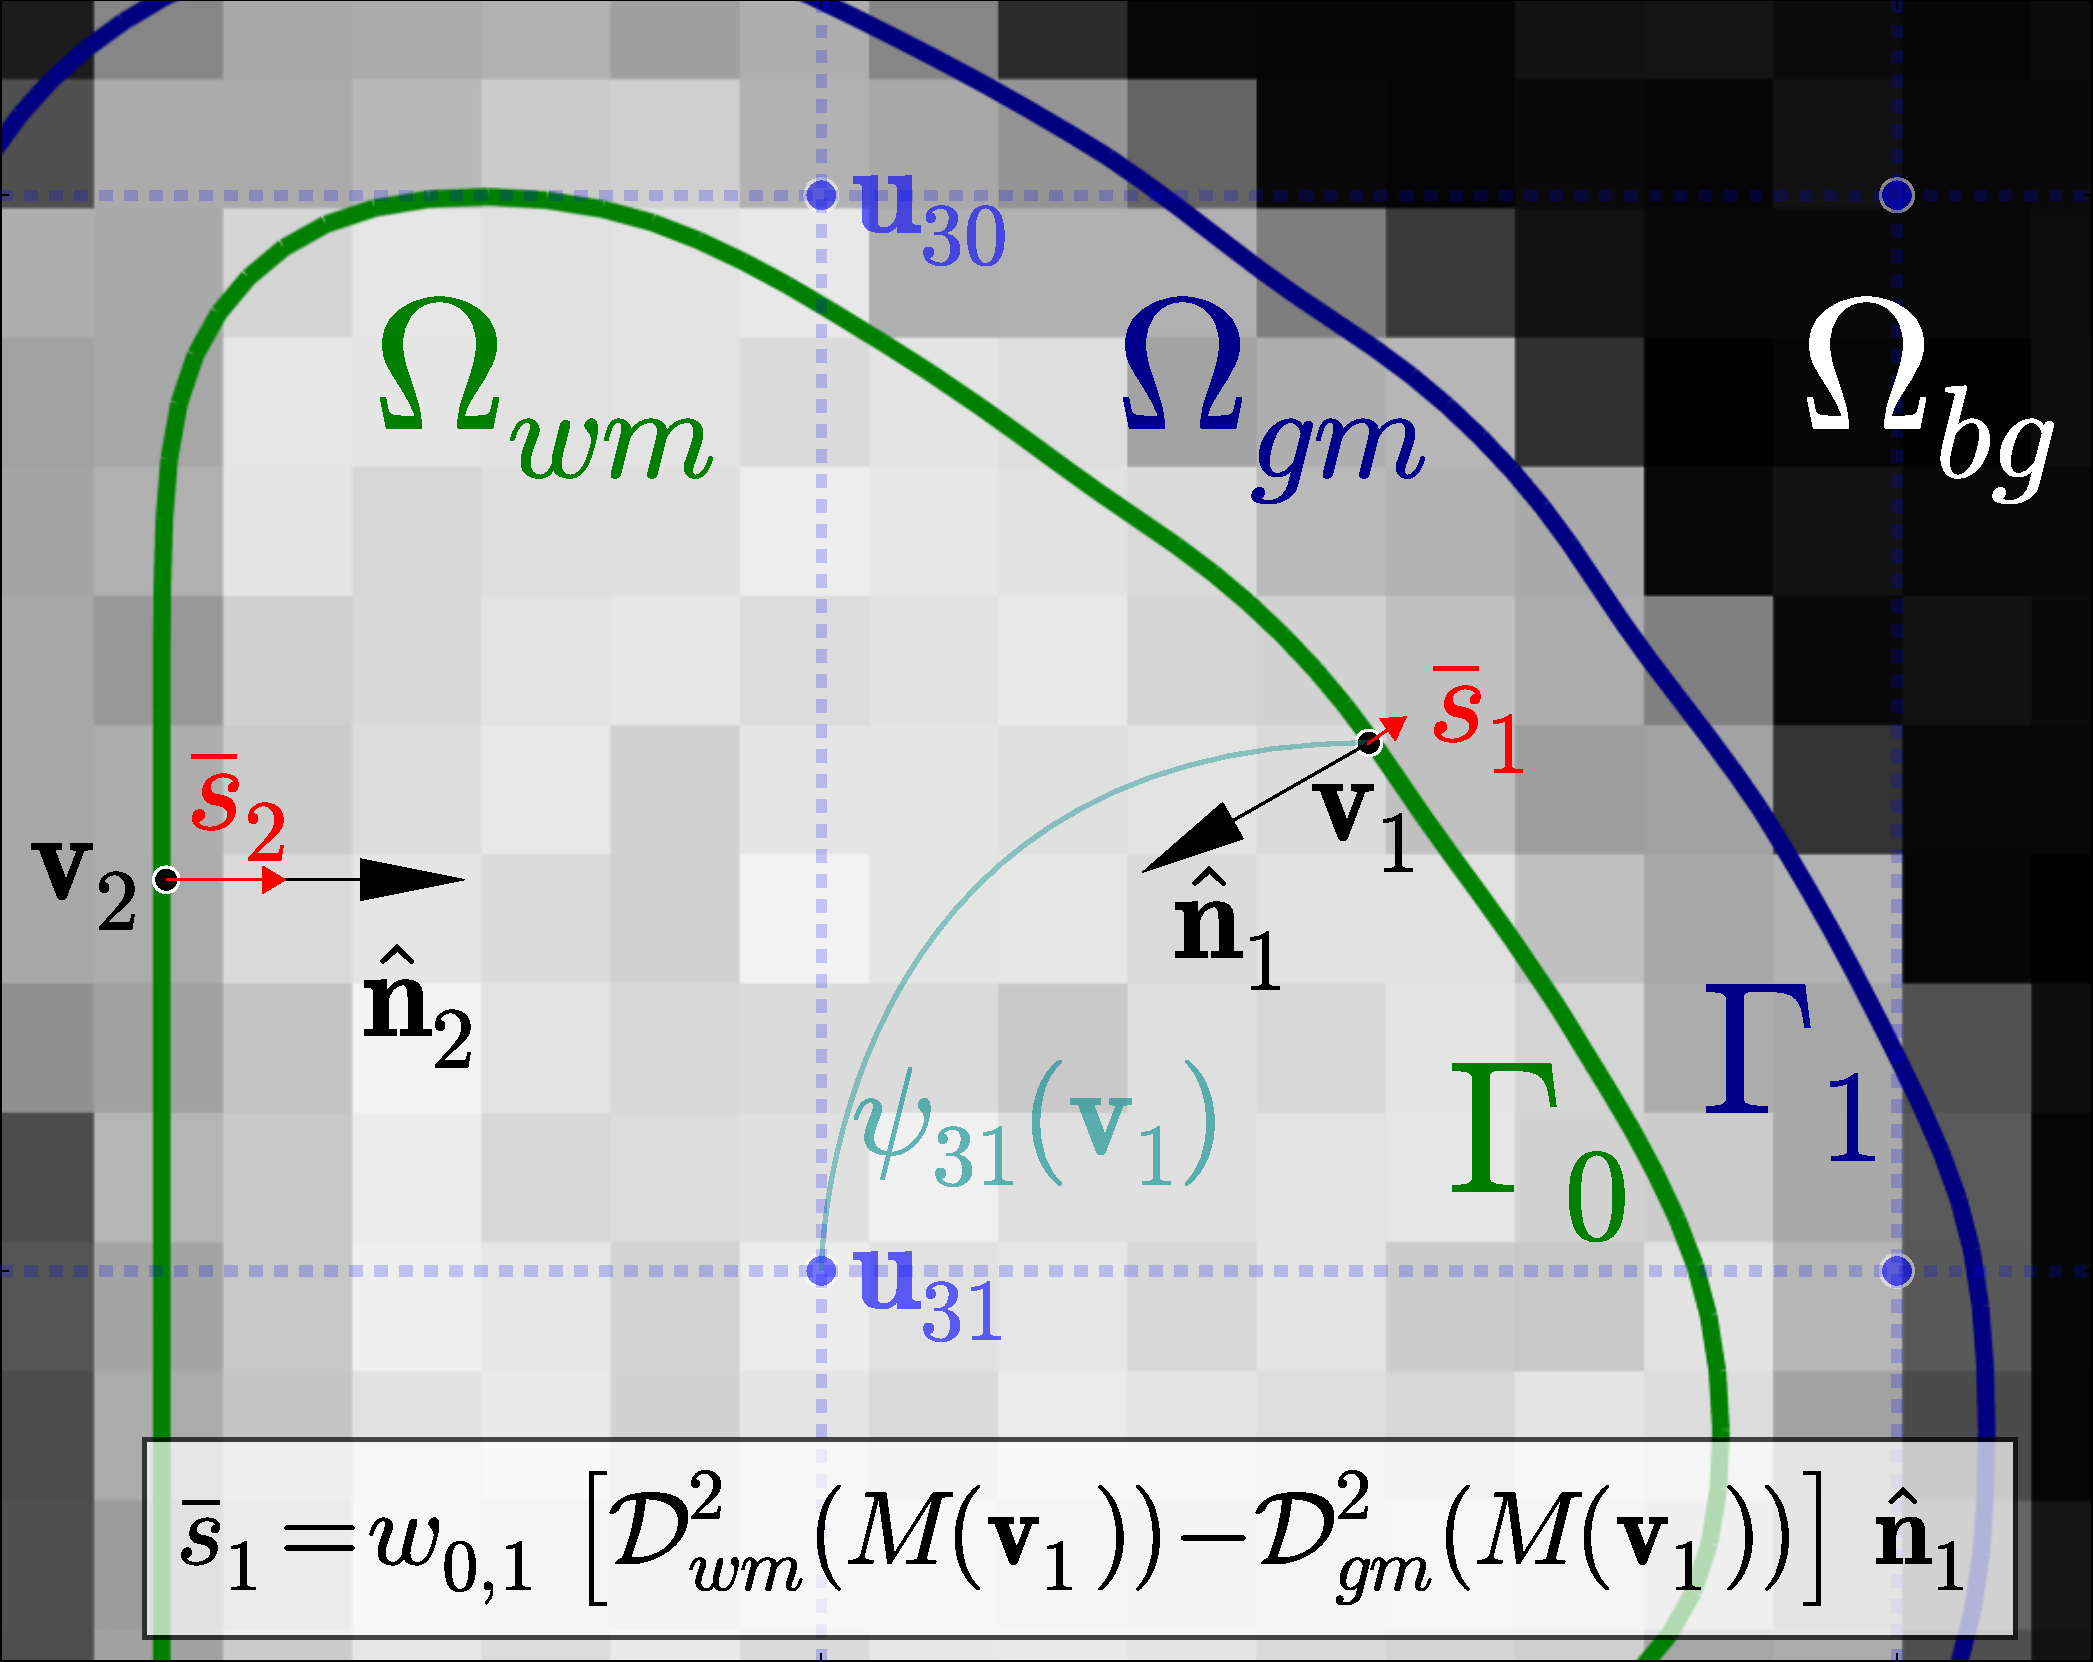
\includegraphics[width=\linewidth]{figures/figure01}
	\caption{The active contours are defined as the interfacing surfaces of the segmenting
	\glspl{roi} $\Omega_i$, and represented in green and dark blue colors in this
	close-up.
	They iteratively through their normals $\hat{n}_i$ at each vertex $\vec{v}_i$ of the mesh.
	The gradient speeds $\bar{s}_i$ are computed as the disparity between data energies of
	the vertex $\vec{v}_i$ in each limiting region as described in \eqref{eq:energy}.
	In this figure, the gradient speed corresponding to $\vec{v}_1$ is written in the lower
	box, $\Omega_{wm}$ being the inner limiting region and $\Omega_{gm}$ the outer.
	Finally, every $\bar{s}_i$ is projected into the grid of control points $\vec{u}_k$ that
	support the deformation field through the corresponding weights $\psi_k(\vec{v}_i)$ obtained
	as in \eqref{eq:basis_derivative}.
	}\label{fig:method}
\end{figure}

\paragraph*{Deformation model}\label{sec:deformation_model}
Let us denote $\{\vec{v}_i\}_{i=1 \ldots N_c}$ the vertices of one or several prior
  surface(s).
In our application, these surfaces are triangularized meshes extracted using \emph{FreeSurfer}
  \citep{fischl_freesurfer_2012}.
The transform $\hat{U}$ \eqref{eq:transform} is supported by a dense deformation field
  $u(\vec{r})$, such that:

  \begin{equation}
  \vec{v}_i' = \hat{U}\{\vec{v}_i\} = \vec{v}_i + u(\vec{v}_i).
  \label{eq:nodes_tfm}
  \end{equation}

Since the nodes of the anatomical surfaces likely lay off-grid, it is required to
  derive $u(\vec{r})$ from a discrete set of parameters $\{\vec{u}_k\}_{k=1 \ldots K}$.
Densification is achieved through a set of associated basis functions $\psi_k$:

  \begin{equation}
  u(\vec{r}) = \sum_k \psi_k(\vec{r}) \vec{u}_k.
  \label{eq:intp_kernel}
  \end{equation}

In our implementation, $\psi_k$ is chosen to be a tensor-product B-Spline kernel
  of degree 3 ($\beta_3$).
Then, introducing \eqref{eq:intp_kernel} into \eqref{eq:nodes_tfm} and replacing
  $\psi$ by the actual kernel function, the transformation writes:

  \begin{equation}
    \vec{v}_i' = \vec{v}_i + \sum_k \left[ \vec{u}_k \, \underset{d}{\prod}
      \beta_3( (\vec{v}_i - \vec{r}_k) \cdot \hat{\mathbf{e}}_d ) \right],
  \label{eq:transformation}
  \end{equation}

  with $\hat{\mathbf{e}}_d$ being the unitary vector along axis $d$.


\paragraph*{Optimization}
\label{sec:gradient_descent}
To find the minimum of the energy functional \eqref{eq:energy},
  we propose a gradient-descent approach with respect to the underlying
  deformation field through the following \gls*{pde}:

  \begin{equation}
  \frac{\partial u(\vec{r},t)}{\partial t} \propto - \frac{\partial E(\vec{u})}{\partial \vec{u}_k},
  \label{eq:general_gradient_descent}
  \end{equation}

  with $t$ being an artificial time parameter of the contour
  evolution, and $\vec{u}_k$ the parameters supporting the estimate
  $\hat{U}$ of the transformation at the current time point.
Now, we introduce \eqref{eq:energy} in \eqref{eq:general_gradient_descent}:

  \begin{align}
  \frac{\partial E(\vec{u})}{\partial \vec{u}_k} &=
  \frac{ \partial }{\partial \vec{u}_k} \Big\{
  \int_{\Omega} \underset{l}{\sum} \mdist{f'}{l} \,d\vec{r} \notag\\
  &+ \int_{\Omega} [ \boldsymbol{\alpha} \cdot u(\vec{r})^{\circ2}
  + \boldsymbol{\beta} \cdot (\nabla \cdot u(\vec{r}))^{\circ2} ] \,d\vec{r}
  \Big\}.
  \label{eq:gradient_descent}
  \end{align}


Therefore, we can apply a discretized interpretation of \eqref{eq:shape_gradients}
  to compute the data term in \eqref{eq:gradient_descent} as follows:

  \begin{align}
  \frac{\partial E_{data}(\vec{u})}{\partial \vec{u}_k} &=
  \frac{ \partial }{\partial \vec{u}_k} \left\{
   \underset{\vec{x} \in \Omega_l}{\sum} \underset{l}{\sum} \mdist{f'}{l} \right\}
  = \underset{i}{\sum}
   \left\langle \frac{\partial \vec{v}_i'}{\partial \vec{u}_k}, \bar{s}_i'\right\rangle,
  \label{eq:gradient_wshape}
  \end{align}

  in this case, the formulation has been adapted to the non-binary case, $\{l,m\}$
  being any pair of neighboring regions, and $\Gamma_{l,m}$ the contour separating
  them such that $\vec{x}' = \vec{v}' \in\Gamma_{l,m} \iff \vec{x}\in \partial\Omega_i \cap \partial\Omega_j$
  and $\vec{n_i}'$ is the unit inward normal to the contour at $c_i'$.


Finally, we can compute:

  \begin{align}
  \frac{\partial \vec{v}_i'}{\partial \vec{u}_k} &= \frac{\partial}{\partial \vec{u}_k}
  \left\{ \vec{v}_i + \sum_k \psi_k(\vec{v}_i) \vec{u}_k \right\}
  = \psi_k(\vec{v}_i)\, \hat{\vec{e}}
  \label{eq:basis_derivative}
  \end{align}

  where $\hat{\vec{e}}$ is the coordinates system's unit vector.
The vertex speeds $\bar{s}_i'$ obtained by computing the shape-gradients \eqref{eq:shape_gradients},
	are then projected to the deformation field in order to obtain the derivatives $\vec{g}_k$
	corresponding to $\vec{u}_k$:

  \begin{equation}
  \vec{g}_{i,k} = \left\langle \frac{\partial}{\partial \vec{u}_k}{\vec{v}_i}', \bar{s}_i'\right\rangle
  = - \left[ \mdist{f_i'}{l} - \mdist{f_i'}{m} \right] \psi_k(\vec{v}_i)\, \hat{\vec{e}},
  \end{equation}

  then the full gradient evolution equation \eqref{eq:gradient_descent} yields:

  \begin{align}
  \frac{\partial E(\vec{u}_k)}{\partial \vec{u}_k} =
  &\underset{i}{\sum} \vec{g}_{i,k} +2\, \boldsymbol{\alpha} \vec{u}_k
  -2\, \boldsymbol{\beta} \Delta \vec{u}_k,
  \label{eq:gradient_final}
  \end{align}

{\color{red} \paragraph*{Evidencing convergence and settings}
discuss choice of $\tau$, Courant-Friedrichs-Lewy (CFL) condition / Wolfe conditions,
multi-resolutions on the bspline grid, image samples and surface sampling,  etc.
}


\subsection*{Experiments and evaluation}
\label{sec:experiments_evaluation}
%
In order to demonstrate the applicability of the registration method, we first
  subjected it to a battery of random tests over synthetic data and then applied
  it on real data.
\autoref{fig:evworkflows} presents the workflow implementing the evaluation instruments.
Besides a visual assessment of the results, we report quantitative evaluations using
  two metrics.
In the case of the phantoms, as we warped data along the three available dimensions,
  we computed the Haussdorf distance, integrating the ``point-to-cell'' method
	implemented by \cite{commandeur_vtk_2011}.
Conversely, the susceptibility-derived distortions only happen along the phase
  encoding axis of the image.
Therefore, a \gls*{swindex} can be computed as the one-to-one distance between corresponding
  vertices of surfaces, weighted by their respective Voronoi area $w_i$:

  \begin{equation}
  sWI = \frac{1}{P} \sum\limits_p^P \frac{1}{A_p} \sum\limits_i^{N_p} w_i\,\|
  \vec{v}_i - \hat{\vec{v}}_i \|
  \end{equation}

  where $\vec{v}_i$ are the locations of the $N_p$ vertices in each $p \in \{1, \dots P\}$
  prior, $A_p$ the total area of surface $p$, and $\hat{\vec{v}}_i$ is the location
  recovered corresponding to the vertex $\vec{v}_i$.


\begin{figure*}
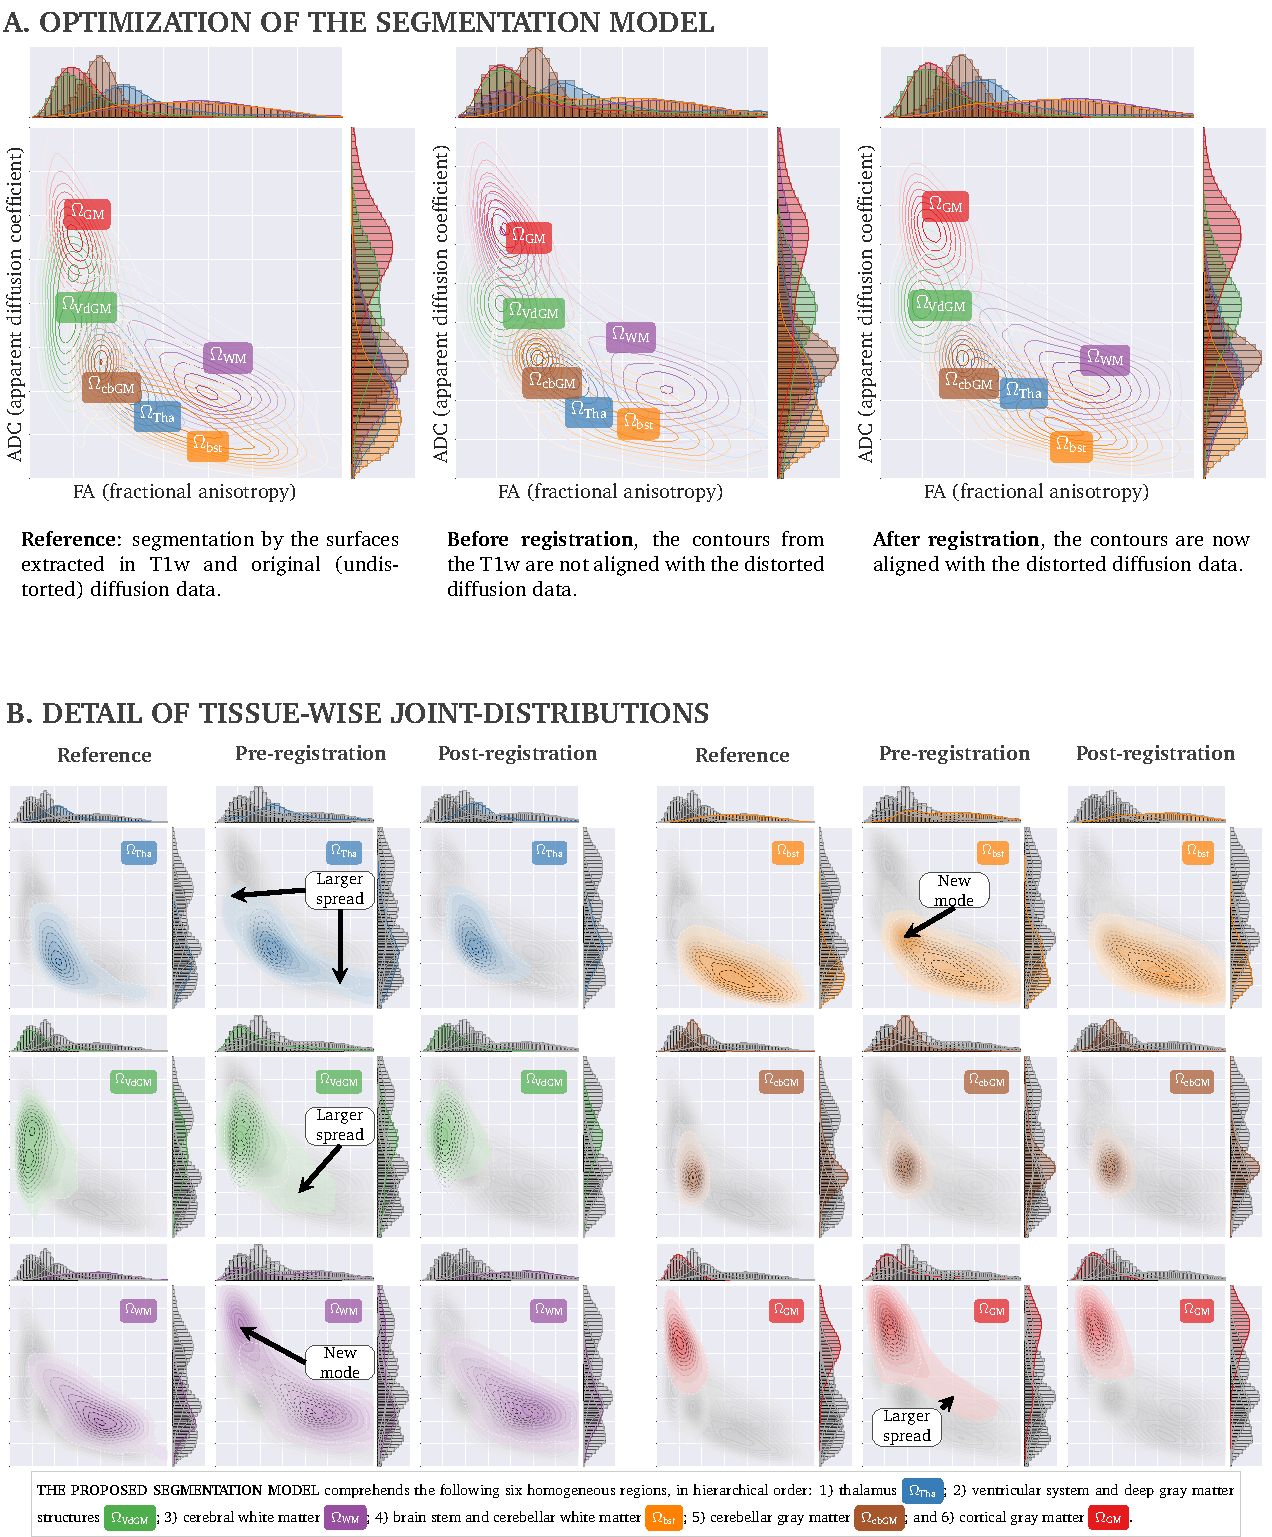
\includegraphics[width=\linewidth]{figures/figure02}
\caption{Experimental workflow applied on real data from the \gls*{hcp}.
  1) The prior surfaces are extracted from the anatomical reference (\gls*{t1} image).
	2) To operate as ground truth, we generate plausible-synthetic distortion $U^{-1}_{true}$
	  from the fieldmap using \eqref{eq:fieldmap}.
	3) The \gls*{dmri} data are warped using $U^{-1}_{true}$ to reproduce the effects of real
	  susceptibility-derived distortions.
	Target diffusion scalars (\gls*{fa} and \gls*{adc}) are computed on the distorted data and
		stacked to feed the multivariate input required by our algorithm.
	4) Registration is run, obtaining a $U_{test} = \hat{U}_{true}$, an estimation of
	  the ground-truth deformation $U_{true}$.
	  A cross-comparison methodology is also applied, to obtain a competing $U_{cc}$.
	5) Results are visually and quantitatively evaluated.}\label{fig:evworkflows}
\end{figure*}

\subsection*{Image Data and preprocessing}
\label{sec:datasets}

\paragraph*{Simulated phantoms}%
\label{sec:digital_phantoms}
We proved the concept on simplistic digital phantoms which we will name after their
  appearance as ``box'', ``ball'', ``L-shape'', and ``gyrus'' (\autoref{fig:phantom},
  boxes A and B).
Using \emph{phantomas} \citep{caruyer_phantomas_2014}, we simulated
  \gls*{t1} (TE/TR=10/1500ms) and \gls*{t2} images (TE/TR=90/5000ms)
  corresponding to each appearance shape, with two resolutions each
  ($1.0mm$ and $2.0mm$ isotropic).
Simulations were corrupted with rician noise for a \gls*{snr} of 300.0.
The reference surfaces were extracted using the marching-cubes algorithm
  shipped with \emph{FreeSurfer} \citep{fischl_freesurfer_2012}
  at the higher resolution (1.0mm isotropic).

\begin{figure*}
	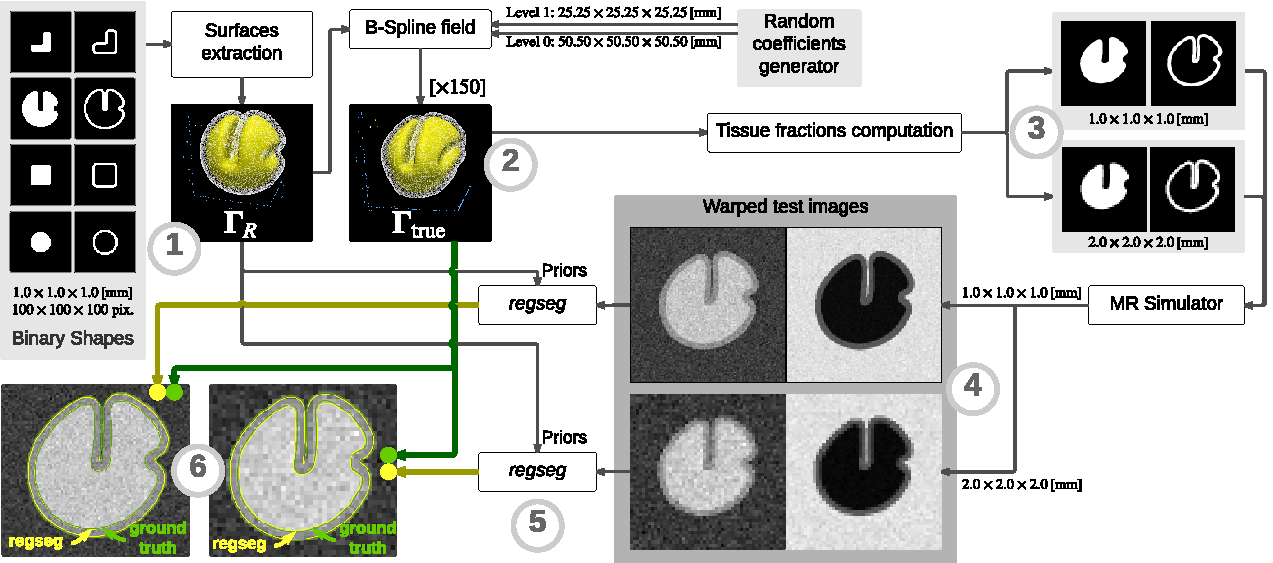
\includegraphics[width=\linewidth]{figures/figure03}
	\caption{A. The ``cortex'' phantom is a spherical shape with two sulci and an
	  outer crust resembling the cortical folding (left).
	The model is used to generate \gls*{t1} and \gls*{t2} images after warping the
	  contours using a random and plausible transformation $U_{true}^{-1}$ (right).
	B. Visual assessment of the results on the low resolution sets:
	  ``gyrus'' (top-left), ``L-shape'' (top-right), ``ball'' (bottom-left),
	  and ``box'' at (bottom-right).
	In yellow color, the recovered contours after registration are represented.
	Our method showed high accuracy, as they are overlapping the ground truth surfaces
	  depicted in green.
	Partial volume effect turns segmentation of the sulci a challenging problem with voxel-wise
	  clustering methods, but it is successfully segmented with our method.
	C. Quantitative evaluation of registration error in terms of average Hausdorff distance of
	  surfaces at high (left) and low (right) resolutions, demonstrating that the error is
	  consistently below the image resolution.
	  }\label{fig:phantom}
\end{figure*}

\paragraph*{Real datasets} %
\label{sec:human_connectome}
%
For the evaluation of the algorithm on real \gls*{dmri} data of human brains,
  we collected 15 datasets from the ``minimally preprocessed''
	 database of the \gls*{hcp}.
We refer the reader to \citep{essen_human_2012} for exact details about acquisition
  parameters, and \citep{glasser_minimal_2013} for the preprocessing issues.
The datasets comprehend a large of images, containing \gls*{t1}, \gls*{t2} and
  multi-shell \gls*{dmri} images.
The original acquisitions are released within ``unprocessed'' packages, and
  the ``minimally preprocessed'' are corrected for artifacts, brain-extracted
  and spatially normalized, along with some results of the standard processing with
  \emph{FreeSurfer}.

Selecting the appropriate labels in the \emph{aparc} segmentation, we applied
  the marching-cubes algorithm again to extract the surface of the following
  six homogeneous regions $\Omega_l$:
  1) the thalamus;
  2) \gls*{csf} of the ventricular system and deep \gls*{gm} structures;
  3) cerebral \gls*{wm};
  4) brain stem and cerebellar \gls*{wm};
	5) cerebellar \gls*{gm}; and
	6) cortical \gls*{gm} surface.
The choice of this particular model of homogeneous regions responds to the joint distribution
  of \gls*{fa} and \gls*{adc} of the human brain, as shown in the {\color{red} Supplemental
  Materials (Figure XX)}.

In this case, we derived the deformation $U_{true}^{-1}$ from the field maps released with
  the corresponding packages of each dataset from the \gls*{hcp} applying \eqref{eq:fieldmap},
  mimicking the real distortions, using a derivation of our previous work
  \citep{esteban_simulationbased_2014}.
After warping the original \gls*{dmri} with $U_{true}^{-1}$, we computed the \gls*{dti} and
  the derived scalars (\gls*{fa} and \gls*{adc}) using \emph{MRtrix} \citep{tournier_mrtrix_2012}.